\documentclass{beamer}
\usepackage{graphicx} % Required for inserting images
\usepackage{float}
\usepackage{amsmath}
\usepackage{amsfonts}
\usepackage{amssymb}
\usepackage{dsfont}
\usepackage{adjustbox}
\usepackage{xcolor}
\newtheorem{exemplo}{Exemplo}
\title{Slides-Estatística para Administração}
\author{ Ismael  Sampaio Bastos}
\date{July 2024}

\begin{document}

\maketitle

\begin{frame}{População x Amostra}

\begin{figure}
    \centering
    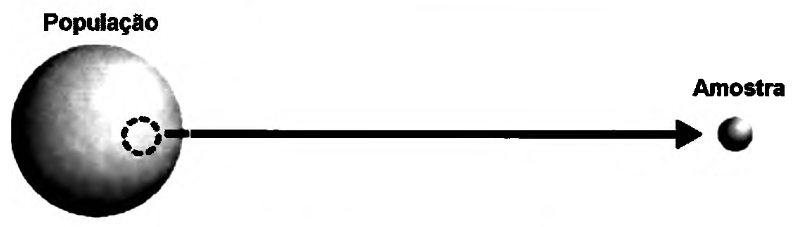
\includegraphics[width=0.7\linewidth]{figures/pop_amostra.png}
\end{figure}
    
\end{frame}

\begin{frame}{População x Amostra}
    O uso de informações de uma amostra para concluir sobre o todo faz parte da atividade
diária da maioria das pessoas. Basta observar como uma cozinheira verifica se o prato
que ela está preparando tem ou não a quantidade adequada de sal.
\end{frame}
    
\begin{frame}{População x Amostra}
    Em geral não temos acesso a informações sobre a população, sendo necessário utilizar uma amostra dessa população. Nesse contexto surge a \textbf{Inferência Estatística}, nos dando ferramentas para estimar informações da população a partir da amostra.
\end{frame}
\begin{frame}{População x Amostra}
Algumas questões ficam em aberto:

\begin{itemize}
    \item Como selecionar essa amostra?
    \item Como determinar qual o tamanho da amostra?
    \item Como realizar inferência a partir da amostra coletada?
\end{itemize}
\end{frame}

\begin{frame}{Estatísticas e Parâmetros}
\begin{itemize}
    \item Parâmetro: Características da população (média, proporção, desvio padrão, etc)
    \item Estatística: Característica da amostra (média amostral, proporção amostral, desvio padrão amostral, etc)
\end{itemize}
    
\end{frame}
\begin{frame}{Amostragem Aleatória Simples}

A amostragem aleatória simples é um dos métodos de amostragem mais comuns e mais utilizados. Podemos obter uma amostra aleatória simples, escrevendo cada elemento da população num cartão, misturando-os numa urna e sorteando tantos cartões quantos desejarmos na amostra

\begin{itemize}
    \item Todos os elementos da população tem a mesma probabilidade de serem selecionados.
    \item Repete-se o experimento até selecionarmos $n$ elementos.
    \item Pode ser com ou sem reposição
    \item $N:$ Tamanho da população, $n:$ tamanho da amostra
\end{itemize}
\end{frame}

\begin{frame}{Estimadores}
    Dizemos que a média amostral é um estimador para a média populacional, a variância amostral é um estimador para a variância populacional, etc. 
    
\end{frame}

\begin{frame}{Distribuição Amostral da Média}
    Temos que a média amostral é dada por:
    $$\Bar{X} = \dfrac{\sum\limits_{i=1}^n X_i}{n}$$

    Perceba que $\Bar{X}$ é uma variável aleatória e portanto tem média (esperança), variância, desvio padrão e uma distribuição de probabilidade.
\end{frame}

\begin{frame}{Distribuição Amostral da Média}
\begin{itemize}
    \item  A distribuição de probabilidade da média amostral é chamada de
distribuição amostral da média.
    \item Conhecer a distribuição amostral de alguma estatística (média,
proporão, variância, etc), bem como suas propriedades, nos
possibilitará fazer afirmações a respeito de quão próximas de, por
exemplo, quão próximas a média da amostra está da média
populacional (ou a variância amostral da variância populacional ou a
proporção amostral da proporção populacional,etc), ou seja, realizar inferência.
\item Em alguns lugares $\Bar{X}$ aparece escrito como sendo $\hat{\mu}$
\end{itemize}

\end{frame}

\begin{frame}{Frame Title}
    
\end{frame}
\end{document}